\documentclass[12pt]{article}
\usepackage{hyperref}
\usepackage{listings}
\usepackage[margin=1in]{geometry}
\usepackage{enumitem}
\usepackage{multicol}
\usepackage{array}
\usepackage{titlesec}
\usepackage{helvet}
\renewcommand{\familydefault}{\sfdefault}
\usepackage{amsmath}     % For math equations
\usepackage{amssymb}     % For advanced math symbols
\usepackage{amsfonts} % For math fonts
\usepackage{gvv}
\usepackage{esint}
\usepackage[utf8]{inputenc}
\usepackage{graphicx}
\usepackage{pgfplots}
\pgfplotsset{compat=1.18}
\titleformat{\section}{\bfseries\large}{\thesection.}{1em}{}
\setlength{\parindent}{0pt}
\setlength{\parskip}{6pt}
\usepackage{multirow}
\usepackage{float}
\usepackage{caption}


\begin{document}

\section*{Problem 9.8.34}
Find the equation of the line passing through the points of intersection of the circles
\begin{align}
3x^2+3y^2-2x+12y-9=0
\quad\text{and}\quad
x^2+y^2+6x+2y-15=0.
\end{align}

\section*{Input Variables (Conic form)}
The general conic is
\begin{align}
\vec{x}^\top V \vec{x} + 2\vec{u}^\top \vec{x} + f = 0, 
\quad \vec{x}=\myvec{x\\y}.
\end{align}

\begin{table}[H]
\centering
\begin{tabular}{|c|c|c|}
\hline
 & $C_1$ & $C_2$ \\
\hline
$V$ & $\myvec{3 & 0 \\ 0 & 3}$ & $\myvec{1 & 0 \\ 0 & 1}$ \\
\hline
$\vec{u}$ & $\myvec{-1 \\ 6}$ & $\myvec{3 \\ 1}$ \\
\hline
$f$ & $-9$ & $-15$ \\
\hline
\end{tabular}
\end{table}

\section*{Solution}

All conics through the intersection points are given by the locus
\begin{align}
\vec{x}^\top (V_1+\mu V_2)\vec{x}
+2(\vec{u}_1+\mu\vec{u}_2)^\top\vec{x}
+(f_1+\mu f_2) &= 0.
\end{align}

Since we want a line, we eliminate the quadratic part by choosing $\mu$ such that
\begin{align}
V_1+\mu V_2 &= (3+\mu)I = 0, \\
\mu &= -3.
\end{align}

Substituting $\mu=-3$, the equation of the required line becomes
\begin{align}
2(\vec{u}_1-3\vec{u}_2)^\top \vec{x} + (f_1-3f_2) &= 0.
\end{align}

Now we compute the coefficients:
\begin{align}
\vec{u}_1-3\vec{u}_2 &= \myvec{-1\\6} - 3\myvec{3\\1} = \myvec{-10\\3}, \\
f_1-3f_2 &= -9 - 3(-15) = 36.
\end{align}

Thus the line is
\begin{align}
2\myvec{-10 & 3}\vec{x} + 36 &= 0.
\end{align}

Multiplying throughout by $-\tfrac{1}{2}$, we obtain
\begin{align}
\myvec{10\\-3}^\top \vec{x} - 18 &= 0.
\end{align}

\begin{align}
\boxed{\myvec{10\\-3}^\top \vec{x} - 18 = 0}
\end{align}

This is the required line through the intersection points.

\begin{figure}[H]
    \centering
    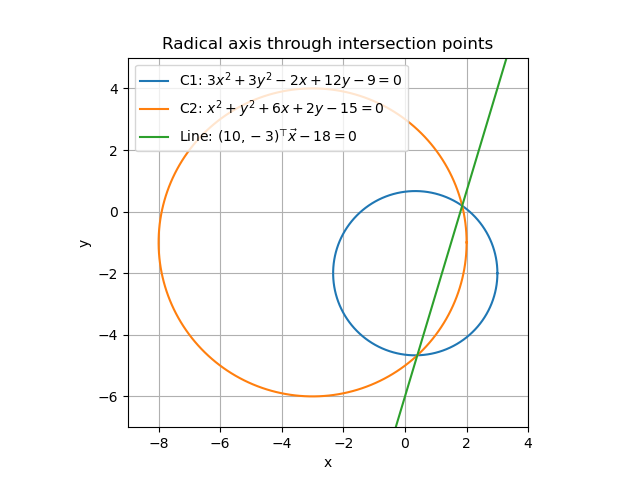
\includegraphics[width=0.9\columnwidth]{figs/radical.png}
    \caption{}
    \label{fig:placeholder}
\end{figure}


\end{document}
